% ------------------------------------------------------------------------------------
\section{Architecture and Theory}\label{sec:arch}
\subsection{One skeleton, three spatial blocks}
All Phase~2 networks share one skeleton (Fig.~\ref{fig:arch}) so that a comparison changes exactly one component.
\begin{enumerate}
\item \textbf{Input projection.} Each sensor's seven features at each step are concatenated with a learned 16-dimensional sensor embedding $\mathbf{e}_i$ (the deep analogue of Phase~1's ``one model per sensor'') and projected to $H=64$ dimensions.
\item \textbf{Temporal encoder.} One GRU~\cite{cho2014gru}, shared by all sensors, reads each sensor's 12 steps and returns its final state $\mathbf{h}_i^{(0)}$ --- a summary of that sensor's last hour (level, trend, missingness).
\item \textbf{Spatial block,} $K$ layers ($K=2$ by default) of one of:
  \emph{none} --- a residual MLP per sensor, same depth and width, no neighbour information (``GRU, no graph'');
  \emph{gcn} --- bidirectional diffusion convolution with the fixed adjacency (``DCRNN-lite''); or
  \emph{gat} --- directed graph attention (``ST-GAT'').
\item \textbf{Head.} An MLP on $[\mathbf{h}_i^{(K)},\mathbf{e}_i]$ outputs three standardised values $\hat z_{i,h}$, turned into mph as $\hat v_{i,h}=b_{i,h}+\sigma_i\hat z_{i,h}$, where $b$ is the sensor's training mean (pure DL) or the XGBoost forecast (hybrid, \S\ref{sec:hybrid}).
\end{enumerate}
We chose ``encode, then propagate'' over running a graph layer at each of the 12 steps: each sensor first summarises its own hour, and the $K$ layers then move those summaries $K$ hops. This is what the LWR analysis asks for --- information about a congestion wave several hops away, including its recent trend --- at one twelfth of the cost of per-step message passing, which matters on CPU.

\subsection{GRU}
For input $\mathbf{x}_s$ and state $\mathbf{h}_{s-1}$: $\mathbf{r}=\sigma(W_r\mathbf{x}_s+U_r\mathbf{h}_{s-1})$, $\mathbf{u}=\sigma(W_u\mathbf{x}_s+U_u\mathbf{h}_{s-1})$, $\tilde{\mathbf{h}}=\tanh(W\mathbf{x}_s+U(\mathbf{r}\odot\mathbf{h}_{s-1}))$, $\mathbf{h}_s=\mathbf{u}\odot\mathbf{h}_{s-1}+(1-\mathbf{u})\odot\tilde{\mathbf{h}}$. The update gate $\mathbf{u}$ lets the cell keep the free-flow level or overwrite it when a drop begins; the gates also mitigate vanishing gradients over the 12 steps.

\subsection{Directed graph attention}
For relation $r\in\{\text{down},\text{up}\}$ with neighbour sets $\mathcal{N}_r(i)$ (plus $i$ itself), head $k$ computes
\begin{align}
e^{r,k}_{ij}&=\mathrm{LeakyReLU}\big(\mathbf{a}^{r,k\top}_{\mathrm{dst}}W^{r,k}\mathbf{h}_i+\mathbf{a}^{r,k\top}_{\mathrm{src}}W^{r,k}\mathbf{h}_j\big)\nonumber\\&\quad+\beta^{r,k}A^{r}_{ij},\\
\alpha^{r,k}_{ij}&=\frac{\exp e^{r,k}_{ij}}{\sum_{l\in\mathcal{N}_r(i)}\exp e^{r,k}_{il}},\\
\mathbf{m}_i&=\big\Vert_{r,k}\textstyle\sum_{j\in\mathcal{N}_r(i)}\alpha^{r,k}_{ij}W^{r,k}\mathbf{h}_j,
\end{align}
followed by $\mathbf{h}_i'=\mathrm{LayerNorm}(\mathbf{h}_i+\mathrm{Dropout}(\mathrm{ELU}(\mathbf{m}_i)))$. Two heads per relation, 32 dimensions per relation. The learnable $\beta$ lets the road-distance weight act as a prior that attention can override. Keeping the two relations separate lets the network learn the LWR asymmetry --- a queue arrives from downstream, a platoon from upstream --- instead of averaging them away. Attention is computed over the edge list (1{,}722 edges per relation including self-loops) rather than all $207^2$ pairs. With $K$ layers each sensor's state depends on sensors up to $K$ hops away (unit-tested), roughly $K\times$1--3~km of road.

\subsection{Diffusion convolution (fixed adjacency)}
With forward and backward random-walk matrices $P_f=D_{\mathrm{out}}^{-1}A$ and $P_b=D_{\mathrm{in}}^{-1}A^\top$, one layer computes $\mathbf{H}'=\mathrm{LN}(\mathbf{H}+\mathrm{ELU}(\mathbf{H}W_0+P_f\mathbf{H}W_1+P_b\mathbf{H}W_2))$ --- a one-step version of DCRNN's bidirectional diffusion~\cite{li2018dcrnn}. Neighbour weights are fixed by road distance; this is the model the brief calls a ``diffusion graph model'' and isolates the value of \emph{learned} attention.

\subsection{Loss}
All models minimise masked MAE in mph, $\mathcal{L}=\frac{1}{|\Omega|}\sum_{(t,i,h)\in\Omega}|\hat v_{t,i,h}-v_{t,i,h}|$, over the observed targets $\Omega$ --- the same quantity used for early stopping and for the Phase~1 headline metric.

\subsection{Hybrid: XGBoost + ST-GAT residual}\label{sec:hybrid}
XGBoost-spatial (Phase~1) is strong on each sensor's own level, daily cycle and one-hop context; its errors are concentrated in congestion onsets, i.e.\ in propagation. The hybrid lets the graph network specialise in exactly that: $b_{t,i,h}=\hat v^{\mathrm{XGB}}_{t,i,h}$, so the network outputs a correction, $\hat v=\hat v^{\mathrm{XGB}}+\sigma_i\hat z$. The network sees the same inputs as ST-GAT.

\emph{Leakage control.} XGBoost's predictions on its own training data are near-perfect in-sample; a residual model trained on them would learn to correct errors that never occur on new data. We therefore generate \emph{out-of-fold} XGBoost forecasts for the training weeks (stacked generalisation~\cite{wolpert1992stacked}): the training period is cut into three contiguous blocks, and for each block 621 per-sensor, per-horizon models are fit on the other two blocks (with one-hour gaps) using the tree counts that Phase~1 early stopping chose, then predict the held-out block. Their out-of-fold MAE (2.81/3.27/3.72) is close to XGBoost's validation MAE (2.70/3.16/3.63), confirming the residuals are realistic. Validation and test forecasts are the unchanged Phase~1 ones; the validation and test weeks are never used to fit XGBoost.

\subsection{Physics-informed variant: soft LWR penalty}
With per-sensor free-flow speed $v_f$ (95th percentile of training speeds), Greenshields' relation gives normalised density $k=1-v/v_f\in[0,1]$ and flow $q=v_f k(1-k)$. Over a horizon of $\Delta t$ hours, conservation of vehicles for sensor $i$ reads
\begin{equation}
r_{i,h}=\hat k_{i,h}-k_{i,0}+\Delta t_h\,\frac{\hat q_{i,h}-\textstyle\sum_{j}\tilde A_{ji}\hat q_{j,h}}{\Delta x_i}\approx 0,
\end{equation}
where $\tilde A_{ji}$ are the row-normalised upstream weights and $\Delta x_i$ the weighted mean road distance to the upstream neighbours. ST-GAT-LWR adds $\lambda\cdot\mathrm{Huber}(r)$ ($\lambda=1$) to the loss. The penalty uses no targets; it asks forecasts to be physically plausible, in the spirit of physics-informed learning~\cite{raissi2019pinn}. It is approximate --- Greenshields is a crude fundamental diagram, sensors are points rather than cells, and on-ramps add unobserved inflow --- so we treat it as a soft prior and let the ablation decide its value.

\subsection{Significance}
To compare two forecasters on the same test samples we use the Diebold--Mariano test~\cite{diebold1995dm}: the loss differential $d_t$ is the difference of network-mean absolute errors at test time $t$; $\mathrm{DM}=\bar d/\sqrt{\hat V/T}$ with a Newey--West variance using $h-1$ lags, since $h$-step-ahead forecast errors are autocorrelated. A negative DM favours the first model.

\begin{figure}[t]\centering
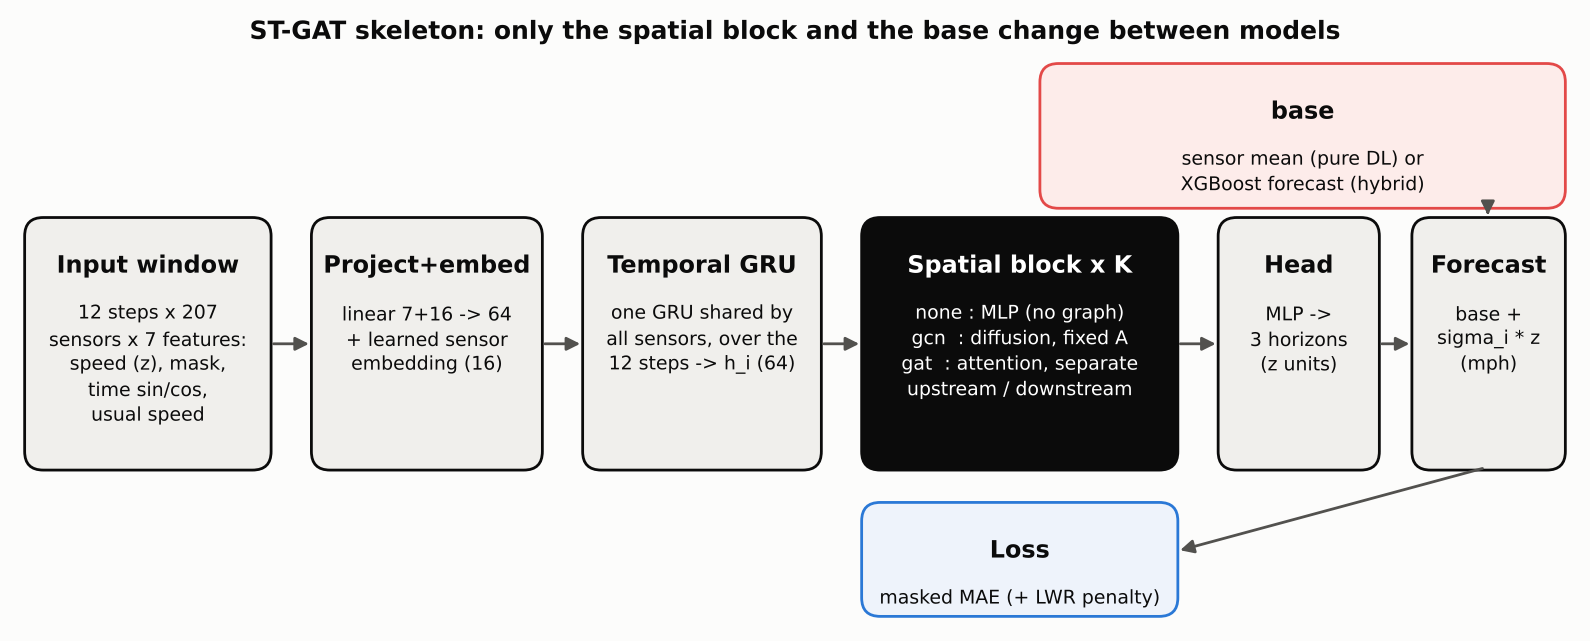
\includegraphics[width=\columnwidth]{fig_dl_architecture}
\caption{Phase~2 skeleton. Only the spatial block changes between the no-graph, diffusion and attention models; the hybrid adds the XGBoost forecast as the base the network corrects.}
\label{fig:arch}
\end{figure}

% ------------------------------------------------------------------------------------
\section{Experimental Setup}
\textbf{Fair comparison.} Same data, masking, split, sample indices, 12-step history, horizons and evaluation code as Phase~1. Phase~1 models are reported from their saved predictions.

\textbf{Training.} AdamW, learning rate $10^{-3}$ ($5\times10^{-4}$ for the hybrid, which starts close to the optimum), batch 64, 8{,}000 random windows per epoch, at most 30 epochs, early stopping with patience 5 on validation masked MAE, best checkpoint restored. Hidden size 64, two graph layers, dropout 0.1. These values were fixed after a short pilot on the validation weeks; the test weeks were scored once, at the end. Everything runs on two CPU cores (no GPU): one main model takes about 40 minutes.

\textbf{Ablations.} To fit the CPU budget, design ablations use a shorter, \emph{identical} budget of 12 epochs and are compared with ST-GAT-short, the main model trained under that same budget. Each changes one thing: number of hops (1/2/3), directed vs undirected edges, the road graph vs a random graph with the same out-degrees and weights, masking vs feeding outages as 0~mph, dropout and weight decay on vs off, and the hybrid with vs without a graph. The two key comparisons --- graph vs no graph, attention vs fixed weights --- use the full budget. Three seeds (12-epoch budget) estimate run-to-run spread.
